% ~~~ [ Profiling ] ~~~~~~~~~~~~~~~~~~~~~~~~~~~~~~~~~~~~~~~~~~~~~~~~~~~~~~~~~~~~

\subsubsection{Profiling}
\label{sec:ver_profiling}

The initial implementation of the LLVM IR lexer (see section~\ref{sec:impl_llvm_ir_library}) focused on correctness, and strived to be as simple and straight forward as possible. Once feature complete and thoroughly tested, the lexer was profiled for the first time and a major performance bottleneck was identified; as illustrated in figure~\ref{fig:lexer_pprof}. When scanning letters, the \texttt{lexLetter} function used a hash map to check if the scanned letters were part of a keyword. As letters make up the majority of the characters in LLVM IR source files, this caused an extensive number of hash map iterations which accounted for roughly 70\% of the total execution time. To fix this issue, a benchmark test was implemented to measure the performance changes between the original and the updated version; as further described in section~\ref{sec:ver_benchmarks}. At this stage, only CPU profiling has been utilised to identify performance bottlenecks. Future work may leverage memory profiling to further improve the performance of the decompilation components.

\begin{figure}[htbp]
	\begin{center}
		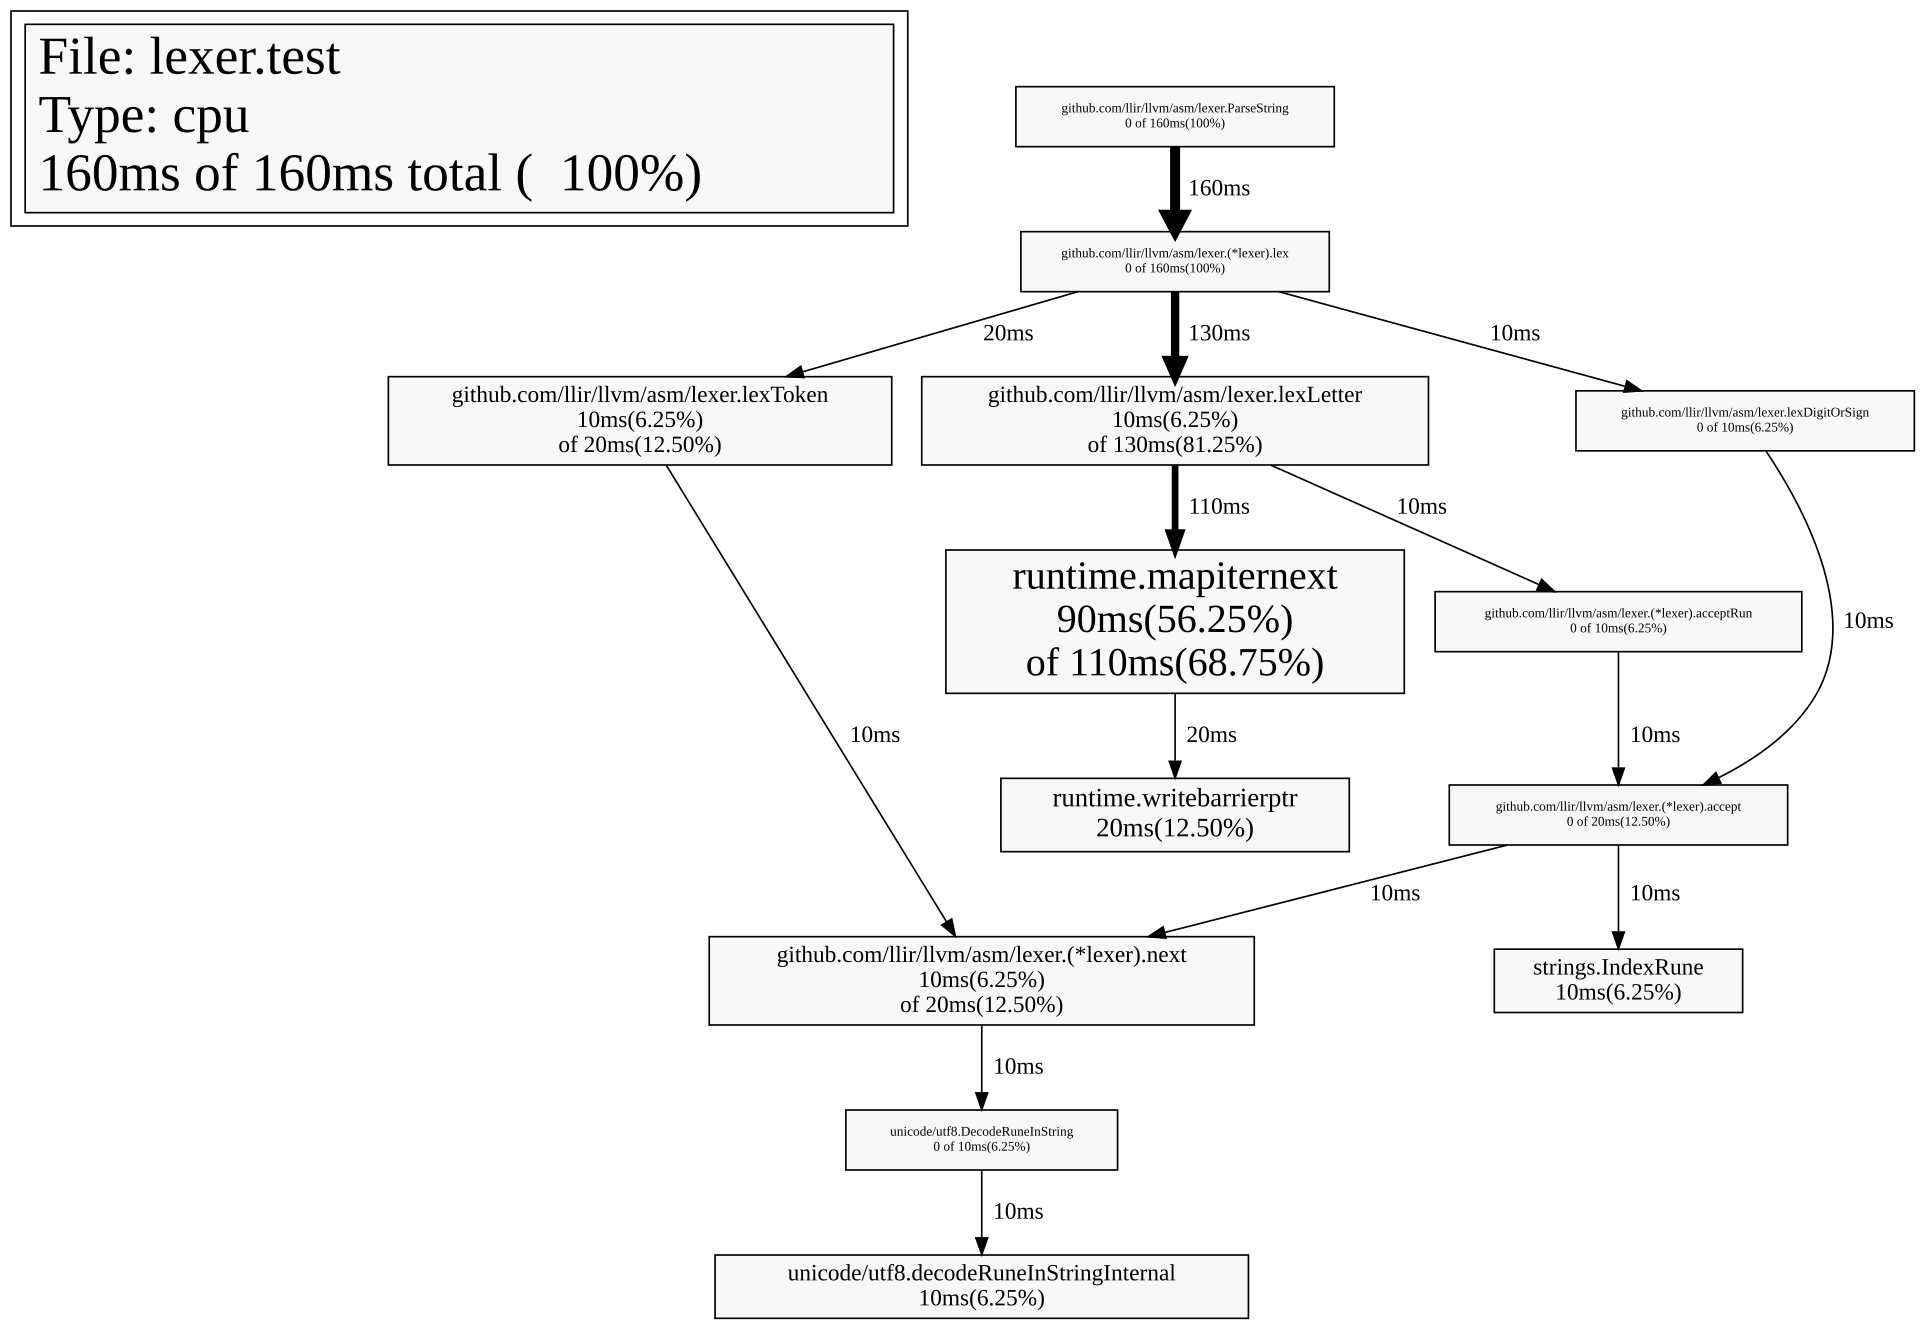
\includegraphics[width=\textwidth]{inc/8_ver/lexer_pprof.png}
		\caption{A major performance bottleneck was located when profiling the LLVM IR lexer for the first time. Roughly 70\% of the total execution time was spent doing hash map iterations (i.e. \texttt{runtime.mapiternext}).}
		\label{fig:lexer_pprof}
	\end{center}
\end{figure}
